\chapter{First-Principles Study of Metallic Uranium}
\textit{A portion of this chapter was published as an article in Computational Material \mbox{Science}. The authors are A. Rafi M. Iasir and Karl D. Hammond of the University of Missouri.}


\section{Introduction}\label{sec_intro}
Uranium is the heaviest naturally-occurring element on Earth. The discovery of
fission in uranium (specifically, in $^{235}$U) impacted not only scientists
and engineers all over the world, it also changed global politics forever. In
nuclear research, the nucleus of the uranium atom is of much more importance
than the electrons surrounding it, but the electronic structure is important
to the thermodynamic properties, including crystal structure. The structural
features are particularly important to the study of next-generation nuclear
fuels, such as \text{U-10Mo}, that are based on metallic uranium.
The electronic behavior of uranium, along with other light actinides (Pa--Pu),
results in a low-symmetry crystal structure at ambient temperature and
pressure---most metallic elements take on relatively high-symmetry structures
(bcc, fcc, and hcp), but the light actinides are either orthorhombic or
monoclinic at standard temperature and pressure.
Pure uranium exists in three different solid phases at atmospheric pressure,
depending on the temperature:
\textalpha\ (base-centered orthorhombic), \textbeta\ (tetragonal) and
\textgamma\ (body-centered cubic). At atmospheric pressure, \textalpha-U
transforms to \textbeta-U at approximately 935~K, and \textbeta-U transforms to
\textgamma-U at approximately
1045~K~\cite{lawson1988structure,akella1997structural}.
The influence of $5f$
electron--electron correlation plays a pivotal role in the crystallographic
behavior of uranium and other light
actinides~\cite{lander2003gh,freemanHandbook1984}; with this in mind, proper
representation of uranium's $5f$ electrons is very important.

The stability of the crystal structures of the inner transition metals has been
the target of several electronic structure studies.
Eriksson and coworkers~\cite{wills1992crystal,eriksson1993first} performed
comparative studies of thorium, protactinium, and uranium's crystal
structures, calculating the equilibrium volume and bulk modulus using the
full-potential linear-muffin-tin-orbital (FP-LMTO) technique and the local
density approximation (LDA)\@. The calculated lattice parameters and
equilibrium unit cell volumes showed good agreement with experiments; the
bulk modulus of protactinium was significantly underestimated, but the values
for uranium and thorium were within the range of experimental values.
Crocombette \etal~\cite{crocombette2001plane} used norm-conserving
pseudopotentials to study three metallic phases of uranium (\textalpha,
\textgamma, and a hypothetical fcc structure). The calculated equilibrium
volume for \textalpha~uranium was underestimated by more than 6~percent.
S{\"o}derlind~\cite{soderlind2002first} calculated the equilibrium lattice
parameters and also estimated the elastic moduli of
\textalpha~uranium using the FP-LMTO method. The calculated equilibrium
lattice parameters were in good agreement with experimental values, but
the elastic moduli did not agree particularly well with experimental
values. The calculated elastic moduli were likely higher than experimental
values because uranium undergoes strong phonon softening with increases in
temperature, and the experimental values (taken at room temperature) would
likely be lower than they would be at low
temperatures~\cite{lawson2000melting}.

S\"oderlind's~\cite{soderlind2002first} was the first attempt to calculate
\textalpha-uranium's elastic moduli. Other theoretical studies of light
actinides prior to 2000 using full-core (\ie, non-pseudopotential-based)
techniques are summarized by Jones \etal~\cite{jones2000theoretical}.
Taylor~\cite{taylor2008evaluation} studied uranium phases using the projector
augmented-wave (PAW) method~\cite{Bloechl1994} with Perdew and Wang's 1991
(PW91) exchange--correlation functional~\cite{Perdew1992a,Perdew1993}. Taylor
investigated \textalpha, bcc, and fcc uranium. The equilibrium lattice
parameters of \textalpha-uranium were within 1\% of experimental
values at 50~K~\cite{barrett1963crystal}. The lattice parameter of
\textgamma-uranium was also in good agreement with experimental values, though
the lattice parameter of fcc uranium was overestimated compared to the value
calculated by Crocombette \etal~\cite{crocombette2001plane}. Xiang
\etal~\cite{xiang2008quantum} used the Perdew--Burke--Ernzerhof (PBE) 
exchange--correlation functional~\cite{Perdew1996b,Perdew1997}
to study the equilibrium volume of the \textalpha~and \textgamma~uranium. He
also studied the bct structure, an approximation of the \textbeta~phase.
Their results were also in good agreement with previous full potential studies
and experimental results.
Li \etal~\cite{li2012structure} also studied the
structure, formation energies, and elastic moduli of \textalpha, \textbeta,
\textgamma, fcc, and hcp uranium using the PW91 exchange--correlation
functional. Their pseudopotential produced reasonably accurate lattice
parameters and cell volumes for \textgamma-uranium and \textalpha-uranium
accompanied by reasonable elastic moduli.
Beeler \etal~\cite{beeler2013first} utilized the PBE
exchange--correlation functional to study uranium, and found similar values
to Li \etal, with the exception of the body-centered tetragonal case
(approximating \textbeta-uranium).


In the present work, we investigate the crystal structure and elastic
properties of metallic uranium with density functional theory (DFT) with a
projector augmented wave (PAW) pseudopotential~\cite{Bloechl1994}. We
investigate four structures of uranium: \textalpha, \textgamma, bct, and fcc.
Our results are compared with previously published electronic structure
calculations and experiments. The electronic densities of
states for all four crystal structures are also calculated. Our results for
\textalpha-uranium are comparable to previous models, but predicted properties
for \textgamma-uranium are, in general, improvements on previously-published
models.


%The projector augmented method (PAW)~\cite{Bloechl1994,kresse1999ultrasoft} is a general approach to the solution of the first principle electronic structure problem. It introduces projectors and auxiliary localized functions. PAW preserves the all-electrons wavefunctions while keeping the pseudopotential approach. In PAW the all electron KS wavefunction is  replaced by smooth pseudo wave function and auxiliary wave function. A comprehensive description of PAW formalism can be found in Bl\"ochl's famous paper~\cite{Bloechl1994}.

%A brief description of PAW formalism is provided in Appendix~\ref{appen_paw}.


\section{Computational Details}\label{sec_comp}
We perform all calculations using density functional theory (DFT) with
plane-wave basis sets as implemented in the software
\textsc{QuantumEspresso}~\cite{giannozzi2009quantum}. We generated a uranium
pseudopotential for use with the Perdew--Burke--Ernzerhof (PBE)
exchange--correlation functional~\cite{Perdew1996b,Perdew1997}.
The projector augmented wave (PAW) pseudopotential-generating software
atompaw~\cite{holzwarth2001projector,tackett2001projector} was used to generate
the PAW pseudopotential for uranium. The same pseudopotential was used for all
subsequent calculations.

One of the major challenges in studying actinides using DFT is how to treat the
large number of electrons. The pseudopotential approach effectively reduces the
number of electrons by modeling the ``core'' as a potential energy surface,
so generating a pseudopotential requires one to choose the number of electrons
that will be treated explicitly. There are two approaches common for uranium:
``small-core'' pseudopotentials and ``large-core'' pseudopotentials. In a
large-core pseudopotential, the valence electrons are the $5f$, $6s$, $6p$,
$6d$ and $7s$ shells (14~electrons). In small-core pseudopotentials, the $5s$,
$5p$, and $5d$ shells are also included, which treats 32 electrons as valence
electrons. Iche-Tarrat and Marsden~\cite{iche2008examining} have discussed this
topic and shown that the explicit treatment of 32 electrons only marginally
improves the performance of DFT at significantly higher computational cost.
The valence electron configuration of uranium used when generating our
pseudopotential was $6s^2 6p^6 7s^2 6d^1 5f^3$ (\ie, it is a large-core
pseudopotential).
The radius of the augmentation region was chosen to be 2.5~bohr,
which we determined by starting from half the experimental nearest-neighbor
interatomic distance in \textalpha-uranium and adjusting based on
energy--volume minimization.
The pseudo-partial waves were generated using the RRKJ
scheme~\cite{rappe1990optimized}, which uses a sum of Bessel functions to
represent the pseudo-partial waves.
A plane-wave cutoff energy analysis was performed and a 50~Ry energy cutoff was
found to be sufficient based on a plot of total energy against cutoff energy.
All calculations were performed on primitive cells using the cell geometries
and coordinates given by Crocombette \etal~\cite{crocombette2001plane} for
\textalpha-uranium, Beeler \etal~\cite{beeler2013first} for bct uranium, and
values from the Structure of Crystals database~\cite{StructureofCrystals} for
all other structures.
Periodic boundaries were applied in all directions.
The Monkhorst--Pack scheme~\cite{pack1977special} was used for Brillouin zone
sampling; the $k$-point meshes were $20\times20\times26$, $20\times20\times20$,
$18\times18\times18$, and $20\times20\times20$ for the \textalpha, bct,
\textgamma, and fcc lattices, respectively. A
Methfessel--Paxton~\cite{methfessel1989high} smearing method (width 0.02~Ry)
was used to integrate the bands at the Fermi level.
To calculate the nine unique elastic moduli of orthorhombic \textalpha-U,
the energy--strain relationship (see appendix~\ref{appen_elalpha}) was used as described by Ravindran
\etal~\cite{ravindran1998density}.
For cubic structures, the elastic moduli were evaluated using
volume-conserving orthorhombic and monoclinic distortions  as described by
Beckstein \etal~\cite{beckstein2001first}.

\section{Results}
The pseudopotential itself is generated by
atompaw~\cite{holzwarth2001projector,tackett2001projector}, which takes as
input the augmentation radius ($r_\text{PAW}$), core radius ($r_\text{core}$),
shape function cutoff ($r_\text{shape}$), matching radius ($r_\text{vloc}$),
valence and core electron configurations, density functional, and the
cutoff radii for each of the partial waves ($r_{c,i}$). We assumed
$r_c = r_\text{PAW}$ for all valence electrons except the $6s$ and $7s$
electrons, for which $r_c$ was adjusted. The cutoff radii are given in
Table~\ref{table:pseudopotential}.
These cutoffs, combined with the choice of density functional and valence
electrons, are sufficient to reproduce the pseudopotential in atompaw.
\begin{table}
  \caption[Parameters used to generate the pseudopotential in
    atompaw]{Parameters used to generate the pseudopotential in
    atompaw~\cite{holzwarth2001projector,tackett2001projector}.}
  \label{table:pseudopotential}
  \centering
  \begin{tabular}{l l}
    \hline
    Cutoff & Value (bohr) \\
    \hline
    $r_\text{PAW}^{}$   & 2.50 \\
    $r_\text{shape}^{}$ & 2.02 \\
    $r_\text{vloc}^{}$  & 1.50 \\
    $r_\text{core}^{}$  & 1.80 \\
    \hline
    $r_{c,i}^{}$ & $r_\text{PAW}$ \\
    \multicolumn{2}{l}{\quad EXCEPT} \\
    $r_{c,6s}^{}$       & 1.50 \\
    $r_{c,7s}^{}$       & 1.50 \\
    \hline
  \end{tabular}
\end{table}

\nomenclature{$r_{PAW}$}{augmentation radius}
\nomenclature{$r_{\text{core}}$}{core radius}
\nomenclature{$r_{\text{shape}}$}{shape function cutoff}



Properties of several uranium phases as calculated with the pseudopotential
presented above are detailed in the rest of this section.

\subsection{\textalpha-Uranium} \label{subsec_alphaU}
Uranium's \textalpha\ phase has a base-centered orthorhombic structure with
space group \textit{Cmcm} (no.~63). The asymmetric unit has uranium atoms at
Wyckoff position $4c$ $\Bigl(0, \pm y, \pm\frac{1}{4}\Bigr)$, where the
position parameter $y$ has been found to be a function of
temperature~\cite{barrett1963crystal}.
At room temperature, the value of $y$ has been measured to be
0.1024~\cite{barrett1963crystal,lander1994solid}. There are four atoms in the
standard unit cell (two in the primitive cell).
%(A20 \textit{Strukturbeircht}) designation and oC4 Pearson symbol.
The \textalpha\ phase is thermodynamically favorable at temperatures below
935~K and pressures up to 100~GPa~\cite{le2003structural,akella1997structural}.
This makes the \textalpha\ phase important to the nuclear energy community
because it is the naturally-occurring phase of uranium. The solid-state physics
community also shows interest in \textalpha-uranium because of certain unusual
characteristics, including charge density wave transitions and
superconductivity.

The total energy as a function of unit cell volume for \textalpha~uranium is
shown in Figure~\ref{fig:alpha}; Table~\ref{table:eq_al} summarizes the
optimized lattice parameters, the distance parameter $y$, and the calculated
elastic moduli, along with results from previously published calculations
and experiments. We confirm that \textalpha-U is the lowest-energy crystal
structure among those we tested. Our pseudopotential predicts an equilibrium
volume of 20.49~\AA$^3$, which is in close agreement with the experimental
value of 20.530~\AA$^3$ (at 50~K)\@. The position parameter $y$ exhibits a
minimum-energy 
value of 0.0986 at the equilibrium volume of 20.49~\AA$^3$.
This trend in $y$ is similar to that observed in the calculations of
Wills and Eriksson~\cite{wills1992crystal}.

Our cell volume results differ from previous calculations using
PAW~\cite{beeler2013first}, which obtained an equilibrium volume of
19.987~\AA$^3$. A Murnaghan~\cite{murnaghan1944compressibility} fit to the
total energy as a function of volume for \textalpha-uranium yielded a bulk
modulus of 132.1~GPa, which is larger than the experimental value of
$104 \pm 2$~GPa~\cite{le2003structural},
but agrees closely with the quantum molecular dynamics (QMD) results of
Hood \etal~\cite{hood2008quantum} (133.5 GPa)
and the diamond anvil cell (DAC) experiments of Yoo \etal~\cite{yoo1998phase},
which reported a bulk modulus of 135.5~GPa. Our pseudopotential-based results
are in close agreement with the all-electron FP-LMTO calculations of
S{\"o}derlind~\cite{soderlind2002first}, which gave an equilibrium volume of
20.67~\AA$^3$ and a bulk modulus of 133.0~GPa. A published PAW-based
pseudopotential from Beeler \etal~\cite{beeler2013first} yields an equilibrium
volume of 19.92~\AA$^3$, which is lower than our result and farther from both
the experimental value and the result from all-electron calculations.

\begin{figure}
	\centering
    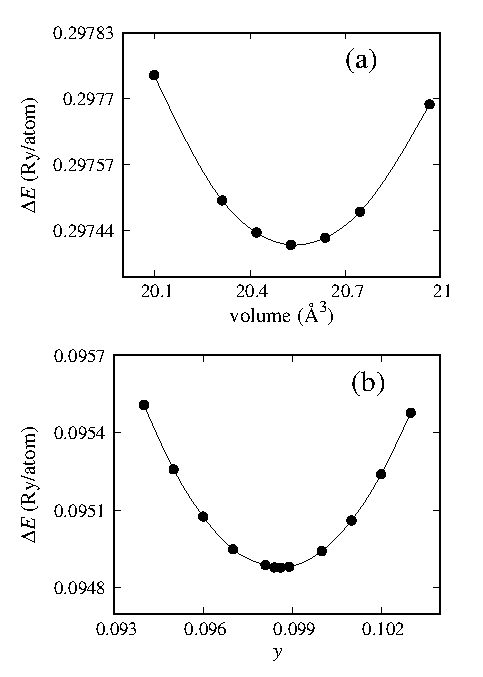
\includegraphics[width=3.25in]{twoPlots_alphaU}
    \caption[Energy vs volume plot for \textalpha-uranium]{(a)~Calculated total energy as a function of volume for
        \textalpha~uranium. (b)~Calculated total energy as a function of the
        positional parameter $y$ for \textalpha~uranium. The calculation of $y$
        is constrained to an equilibrium volume of 20.49~\AA$^3$.}
	\label{fig:alpha}
\end{figure}
 
\begin{table}
\small
%\label{table:eq_al}
\caption[Comparison of ground-state properties and elastic moduli of \textalpha-U with previous work]{Ground-state properties and elastic moduli of \textalpha-U from present work, compared with the PAW pseudopotential calculations of Beeler \etal~\cite{beeler2013first}, the full-core calculations of S{\"o}derlind~\cite{soderlind2002first}, and experiments from Barrett~\cite{barrett1963crystal}, Le Bihan \etal~\cite{le2003structural}, and Fisher and McSkimin~\cite{fisher1958adiabatic}~(295~K).}
\label{table:eq_al}
%\begin{ruledtabular}
\begin{tabular}{cccccccc}
  \hline
    & \multicolumn{3}{c}{Theory}
    && \multicolumn{3}{c}{Experiment} \\
    \cline{2-4}\cline{6-8}
				 & present work  & Beeler~\cite{beeler2013first}  & S{\"o}derlind~\cite{soderlind2002first} && Barrett~\cite{barrett1963crystal} & Le Bihan~\cite{le2003structural} & Fisher~\cite{fisher1958adiabatic} \\ \hline 
$a$ (\AA)		 & 2.834		 & 2.793		 & 2.845	&&	2.836	& 2.8553 & -	\\
$b$ (\AA)		 & 5.862		 & 5.849		 & 5.818	&&	5.867	& 5.8702 & -	\\
$c$ (\AA)		 & 4.932		 & 4.893	     & 4.996	&&	4.936	& 4.9568 & -	\\
$y$ 			 & 0.0986		 & 0.097		 & 0.103	&&	0.102	& 0.102	 & -	\\
volume/atom (\AA$^3$) & 20.48		 & 19.987		 & 20.674	  && 20.535	& 20.770 & -	\\ 
$B$ (GPa)		 & 132.1		 & 151			 & 133		  && -		& 104(2) 	& -	\\
$B'$			 & 5.27			 & -			 & 5.4		  && -		&6.2		& -	\\
$C_{11}$ (GPa)		 & 315			 & 299			 & 300		  &&	-		&-		& 215 \\
$C_{22}$ (GPa)		 & 213			 & 231			 & 220		  &&	-		&-		&199 \\
$C_{33}$ (GPa)		 & 387			 & 364			 & 320		  &&	-		&-		&267 \\
$C_{44}$ (GPa)		 & 135			 &100			 & 150		  &&	-		&-		&124 \\
$C_{55}$ (GPa)		 & 87			 & 150			 & 93		  &&	-		&-		&73 \\
$C_{66}$ (GPa)	     & 104			 & 132			 & 120		  &&	-		&-		&74\\
$C_{12}$ (GPa)		 & 58			 & 59			 & 50		  &&	-		&-		&46\\
$C_{13}$ (GPa)		 & 45			 & 30			 & 5		  &&	-		&-		&22\\
$C_{23}$ (GPa)		 & 146			 & 144			 & 110		  &&	-		&-		&108\\
  \hline
\end{tabular}
%\end{ruledtabular}
\end{table}

The elastic moduli predicted by our pseudopotential are
presented in Table~\ref{table:eq_al}. Like all materials with
orthorhombic symmetry, \textalpha-U has nine unique elastic
moduli. Our model overestimates most of the elastic moduli
relative to experiments. The three primary-direction elastic
moduli ($C_{11}$, $C_{22}$, and $C_{33}$) show good agreement
with other theoretical results and with experiment, though all
three principal elastic moduli are overestimated.
The order ($C_{33} > C_{11} > C_{22}$) of these three elastic
moduli is also consistent with experiments. For $C_{55}$ and
$C_{13}$, the present results also show good agreement with
experiments.  The value of $C_{66}$ is overestimated relative to
experiment, but closer than any existing prediction from a
pseudopotential-based calculation. The other elastic moduli are
generally similar to existing theoretical predictions.

\subsection{\textgamma-U: Crystal Structure and Elastic Moduli}
\label{subsec_gamma}

\begin{table}
%\label{table_eq_gamma}
\caption[Comparison of ground-state properties and elastic moduli of \textgamma-U with previous work]{The equilibrium lattice parameters and volume per atom of \textgamma-uranium. Results are compared with the PAW pseudopotential calculations of Beeler \etal~\cite{beeler2013first} and Taylor~\cite{taylor2008evaluation}, as well as the norm-conserving pseudopotential calculations of Crocombette \etal~\cite{crocombette2001plane} and the experiments of Wilson and Rundle~\cite{wilson1949structures} at room temperature. Elastic moduli are compared with previous PAW pseudopotential calculations from Beeler \etal~\cite{beeler2013first} and Taylor~\cite{taylor2008evaluation}.}
\label{table_eq_gamma}
\footnotesize
%\begin{ruledtabular}
\begin{tabular}{cccccccc}
  \hline
  & \multicolumn{4}{c}{Theory} && \multicolumn{2}{c}{Experiment} \\
  \cline{2-5}\cline{7-8}
			& present work & Beeler~\cite{beeler2013first} & Taylor~\cite{taylor2008evaluation} & Crocombette~\cite{crocombette2001plane} && Wilson~\cite{wilson1949structures} & Yoo~\cite{yoo1998phase} \\ \hline
$a$~(\AA)			&   3.45	   & 3.427	& 3.43	 & 3.37		   && 3.47	&-			\\		
volume/atom~(\AA$^3$) & 20.56		   & 20.124	& 20.18	 & 19.14	   && 20.89	&-			\\ 
$C_{11}$ (GPa) &	40		   & 86		& 161	 & -	&&-	&-	\\ 
$C_{12}$ (GPa) &	145		   & 155	& 184	 & -	&&-	&-	\\
$C_{44}$ (GPa) &   42		   & 37		& 56	 & -	&&-	&-	\\ 
$B$ (GPa)		&  110		   & 132	& 176	 & 170	&&-	& 113.3	\\ \hline
\end{tabular}
%\end{ruledtabular}
\end{table}

The structure of \textgamma-uranium at high temperature was first
elucidated by Wilson and Rundle~\cite{wilson1949structures} at Iowa
State University in 1949 using powdered uranium at
800~\textdegree C\@. The \textgamma~phase of uranium has a
body-centered cubic (bcc; Structurbericht designation A2) structure
with two atoms in the standard unit
cell~\cite{yakel1973review,nashchemistry}.
%(space group $Im\overline{3}m$)
It is thermodynamically stable from 1050~K to the melting point of
1406~K~\cite{yoo1998phase}.

In the nuclear fuels community, \textgamma~uranium is preferred to
\textalpha-uranium because it undergoes isotropic thermal expansion
and radiation-induced swelling~\cite{kittel1993history}. 
As Wilson and Rundle observed~\cite{wilson1949structures},
it is not possible to quench pure \textgamma-uranium to room
temperature, but a metastable bcc phase can be retained at room temperature
in U--Mo alloys.
Recently, it was found that the bcc structure can be retained by alloying
uranium with other metals, such as platinum, palladium, niobium, and
zirconium~\cite{kim2016superconductivity}.
In particular, the eutectoid point of \textgamma-uranium with molybdenum
impurities is at approximately 89~weight-percent uranium; to take advantage of
the depressed phase transition temperature (and the associated increase in
stability of the bcc phase), uranium alloyed with 10~wt\% molybdenum
($\approx$~21.6 at.\%; U-10Mo) is currently being developed as a potential
high-density low-enrichment uranium (LEU) fuel for high-performance research
reactors. The lattice parameters, volume per atom, and elastic moduli as
calculated with our pseudopotential-based model are presented in
Table~\ref{table_eq_gamma}.

The lattice parameters for \textgamma-uranium as calculated with the
pseudopotential presented here are in good agreement with experiments.
The elastic moduli are comparable with those of
Beeler \etal~\cite{beeler2013first} and Taylor~\cite{taylor2008evaluation}.
The value of $C_{12}$ is larger than that of $C_{11}$, which is
a violation of one of the stability criteria for cubic crystals
$(C_{11}-C_{12} > 0)$, often called the Born stability
criteria~\cite{born1940stability,born1954dynamical,Mouhat2014}. This violation
is expected, as the bcc phase of uranium is unstable at low temperatures. The
experimental value of bulk modulus by Yoo \etal~\cite{yoo1998phase} is in good
agreement with our result.

\subsection{Body-centered Tetragonal Uranium}
\label{subsec_bct}

\begin{table}
%\label{table:eq_bct}
\caption[Comparison of ground-state properties and elastic moduli of bct uranium with previous work]{The optimized lattice parameters (\AA), volume per atom (\AA$^3$) and elastic moduli of bct uranium. Our calculated results are compared with those of Beeler \etal~\cite{beeler2013first}, Li \etal~\cite{li2012structure},
Xiang \etal~\cite{xiang2008quantum}, and S\"oderlind~\cite{Soderlind1998}.}
\label{table:eq_bct}
%\begin{ruledtabular}
\begin{tabular}{cccccc}
  \hline
		& present work & Beeler~\cite{beeler2013first} & Li~\cite{li2012structure} & Xiang~\cite{xiang2008quantum} & S\"oderlind~\cite{Soderlind1998} \\ \hline
$a$ (\AA)		&   3.44	   & 3.695	& 3.72 & - & -\\
$c/a$	&	0.8125	   & 0.8	& 1.24 & - & 0.82 \\
volume/atom (\AA$^3$)& 20.44	   & 20.268 & 31.896 & 20.5 & - \\
$C_{11}$ (GPa) &  270		   & 264	& 230 & - & -	\\
$C_{33}$ (GPa) &  257		   & 254	& 204 & - & -	\\
$C_{12}$ (GPa) &  65		   & 55		& 61 & - & -	\\
$C_{13}$ (GPa) &	32		   & 68		& 61 & - & -	\\
$C_{44}$ (GPa) &	59		   & 56		& 79 & - & -	\\
$C_{55}$ (GPa) &	71		   & 56		& 39 & - & - \\
$B$ (GPa)    &	115.4	   & 130	& 114  & - & - \\
  \hline
\end{tabular}
%\end{ruledtabular}
\end{table}
The \textbeta-phase of uranium is stable at atmospheric pressure between 935
and 1045~K~\cite{lawson1988structure}.
Tucker~\cite{tucker1950approximate} determined that it has a tetragonal
structure with 30~atoms per unit cell, but his space group assignment was
later disputed. The assignment of a space group remained a controversy until
1988, when Lawson and coworkers~\cite{lawson1988structure} published neutron
powder diffraction results.
The experimental difficulties lie in the preparation of a single crystal of
\textbeta-uranium and the need to operate at high temperature.
Single crystals of a \textbeta-uranium alloy containing 1.4~atom\% chromium
were created by Tucker~\cite{tucker1951crystal} and quenched to room
temperature, but he did not establish whether this alloy had the same crystal
structure as pure \textbeta-uranium~\cite{lawson1988structure}. An overview of
the development of the crystal structure of \textbeta-uranium is given by
Donohue and Einspahr~\cite{donohue1971structure, donohue1974structures}. The
present consensus is that \textbeta-uranium has a tetragonal crystal structure
with with space group $P4_2/mnm$ (no.~136) and 30~atoms in the unit cell.

We chose to simulate a body-centered tetragonal structure instead of
\textbeta~uranium because of the latter's complexity and computational expense.
A similar simplification was used in studies similar to
ours~\cite{beeler2013first,li2012structure}.
The bct structure has only two atoms per unit cell, and is therefore less
computationally expensive than \textbeta~uranium.
The equilibrium lattice parameters of bct~uranium are presented in
Table~\ref{table:eq_bct}, alongside values from Beeler
\etal~\cite{beeler2013first} and Li \etal~\cite{li2012structure}.
The volume per atom agrees well with Beeler \etal\ but is significantly
different from that of Li \etal.
Xiang \etal~\cite{xiang2008quantum} also studied the bct structure of uranium,
though they did not provide the equilibrium lattice parameter or $c/a$ ratio;
their value of the equilibrium volume per atom was 20.5~\AA$^3$, similar but
larger than our value. Our $c/a$ ratio is in good agreement with
both Beeler \etal~\cite{beeler2013first} (0.8) and
S\"oderlind~\cite{Soderlind1998} (0.82).

\subsection{Face-centered Cubic Uranium}
\label{subsec_fcc}

\begin{table}
%\label{table:eq_fcc}
\caption[Comparison of ground-state properties and elastic parameters of fcc uranium]{The equilibrium lattice parameter, volume per atom, and elastic moduli
of fcc uranium. Results are compared with PAW pseudopotential calculations of
Beeler \etal~\cite{beeler2013first}, Taylor~\cite{taylor2008evaluation}, and
Crocombette \etal~\cite{crocombette2001plane}.}
\label{table:eq_fcc}
%\begin{ruledtabular}
\begin{tabular}{cccccc}
  \hline
				   & present work & Beeler~\cite{beeler2013first} & Taylor~\cite{taylor2008evaluation} & Crocombette~\cite{crocombette2001plane} \\ \hline
$a$ (\AA)				   & 4.300  		  & 4.433	& 4.48	 & 4.30				\\
volume/atom (\AA$^3$)	   & 21.765   & 21.774	& 22.48  & 19.88			\\ 
$C_{11}$ (GPa) &  	67			& 46	 & 184 &-	  \\
$C_{12}$ (GPa) &	130			& 144	 & 267 &-	  \\
$C_{44}$ (GPa) &	38			& 40	 & 28  &-   \\
$B$ (GPa)		&	108.7		& 111	 & 239	&148	\\
  \hline
\end{tabular}
%\end{ruledtabular}
\end{table}
Face-centered cubic uranium does not exist in nature, but it is a reasonable
way to check the pseudopotential. Beeler \etal~\cite{beeler2013first} and
Taylor~\cite{taylor2008evaluation} studied this structure as well, so we
compare our results with theirs.
Table~\ref{table:eq_fcc} shows the equilibrium parameters and elastic moduli
as calculated with our model and with several other published pseudopotentials.
Our results are in good agreement with other pseudopotential calculations,
particularly those of Beeler \etal~\cite{beeler2013first};
the bulk modulus shows good agreement with their value as well.
It should be noted that $C_{12}$ is still higher than $C_{11}$, confirming that this model predicts the fcc phase to be unstable.

\subsection{Electronic Density of States}
\begin{figure}
	\centering
	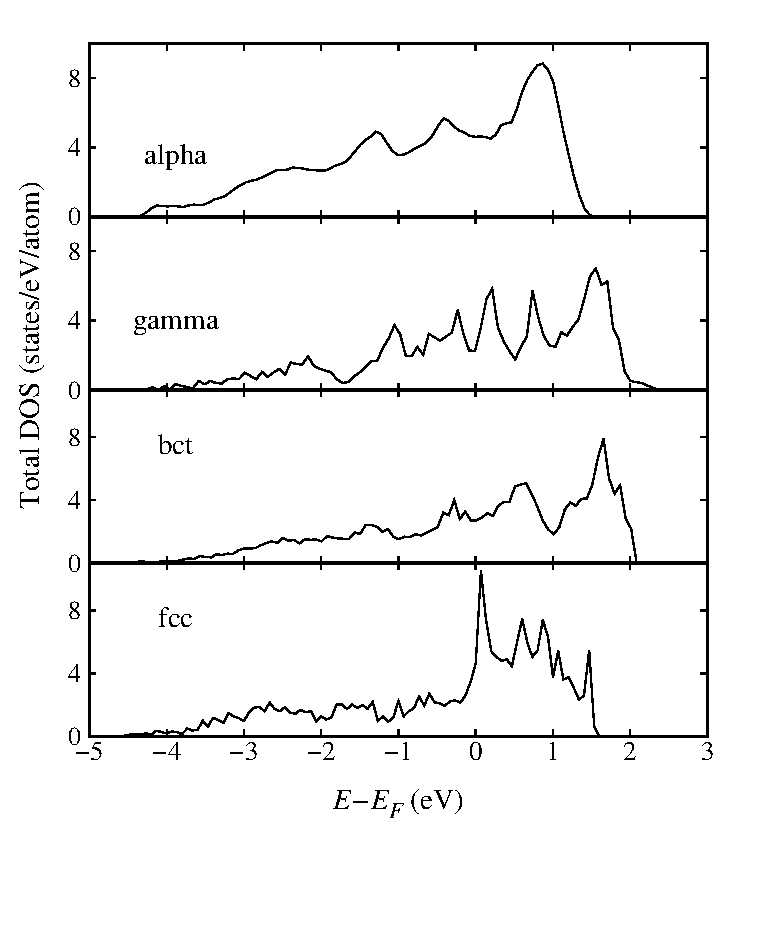
\includegraphics[width=3.25in]{total_DOS_allU}
    \caption{Total electronic densities of states of \textalpha, \textgamma,
      bct, and fcc uranium near the Fermi level.}
	\label{fig:totDos}
\end{figure}

\begin{figure}
	\centering
	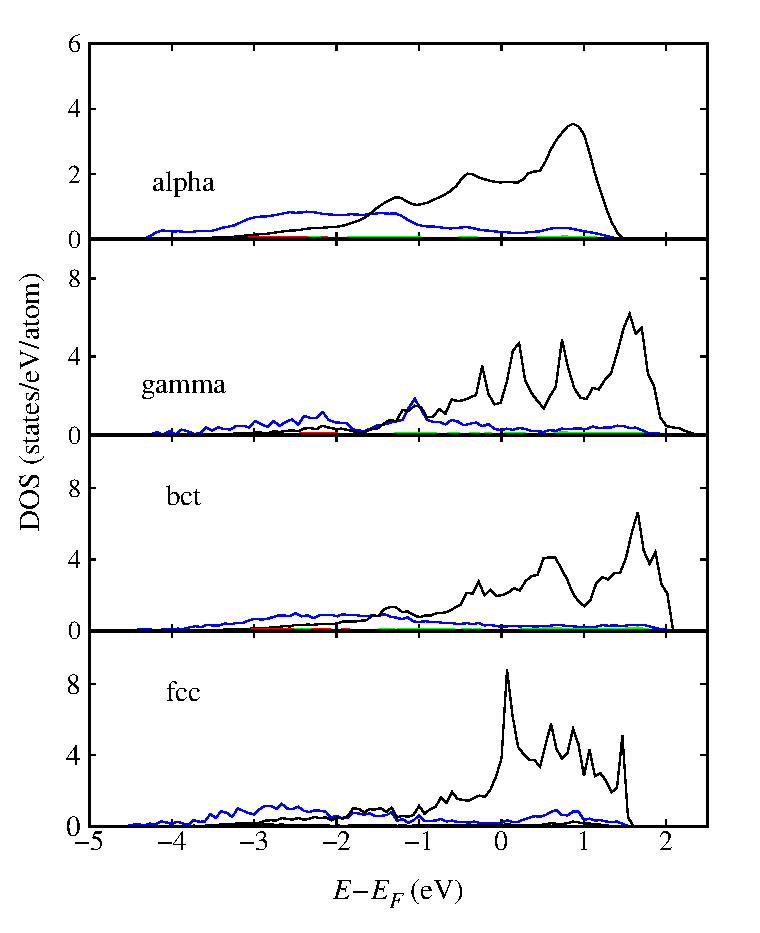
\includegraphics[width=3.25 in]{spdf_orbital}
    \caption[The partial electronic densities of states of \textalpha,
      \textgamma, bct, and fcc uranium near the Fermi level.]{The partial electronic densities of states of \textalpha,
      \textgamma, bct, and fcc uranium near the Fermi level. The $6d$ (blue
      line) and $5f$ (black line) electronic orbitals are shown. The $s$ (red)
      and $p$ (green) electronic orbitals are also included, but due to their
      very low contributions near the Fermi level, they are barely visible.}
	\label{fig:fdorbitals}
\end{figure}

The electronic densities of states (DOS) of \textalpha, bct, \textgamma, and
fcc uranium are shown in Figure \ref{fig:totDos}. The partial densities of
states for the $5f$ and $6d$ orbitals are shown in Figure~\ref{fig:fdorbitals}.
We have only shown the partial densities of states for the $5f$ and $6d$
orbitals because these are the dominant orbitals near the Fermi level of
uranium. There are also contributions from $6s$, $6p$, and $7s$ orbitals near
the Fermi level, but these contributions are not as significant as the dominant
$5f$ and $6d$ orbitals.
%At the Fermi level, the dominant electronic contributions are from the $5f$
%orbitals, though the $6d$ orbitals do contribute.
Electrons near the Fermi level
are important because they are responsible for most of the metallic behavior.
From Figure~\ref{fig:totDos}, it can be seen that the DOS spreads over energies
between $-4$~eV and 2~eV relative to the Fermi level. The density of states
with our model is comparable to those calculated by Beeler
\etal~\cite{beeler2013first} and Xiang \etal~\cite{xiang2008quantum}.
For bcc and bct uranium, the $f$ orbitals spread over a broader range of
energies near the Fermi level and show multiple peaks above the Fermi level.
The high density of states at energies above the Fermi level in the bct
and \textgamma\ phases suggest that these phases would be favored over
\textalpha-uranium at high temperature.

\section{Conclusion}
The equilibrium structures, cell volumes, and elastic moduli have been
calculated using DFT with a newly parameterized pseudopotential model for four
different uranium phases (\textalpha, \textgamma, body-centered
tetragonal, and face-centered cubic). Our results are either in good agreement
with previous work or show improvement in comparison with experiments.
Studying pure uranium is the first step in exploring different alloys of
uranium that are of interest to the nuclear fuels community.
Due to the lower cutoff energies that can typically be used, PAW-based
pseudopotentials allow one to study larger supercells, which in turn provide
more accurate studies of vacancy formation, grain boundaries, and fission gas
transport.

According to our pseudopotential, \textalpha-uranium is the lowest-energy
crystal structure of the ones tested.
The calculated elastic moduli show good agreement with previous DFT studies
and experiments. Our model shows good agreement with previous pseudopotentials,
but generally provides results that are either comparable to previously
published pseudopotentials or closer to experimental values than previously
published pseudopotentials.
The three elastic moduli associated with shear ($C_{44}$, $C_{55}$, and
$C_{66}$) show better agreement with experimental results than the tensile
components. The lattice parameters of the bct structure are also very similar
to those predicted by Beeler \etal~\cite{beeler2013first}, but they deviate
significantly from those of Li \etal~\cite{li2012structure}.
The elastic moduli show very similar trends to previously published models,
apart from $C_{23}$, which is over-predicted by our model.

For \textgamma~uranium, which is of great interest for the development of
low-enrichment uranium fuel, the lattice parameters are in close agreement with
those of of Taylor \etal~\cite{taylor2008evaluation} and with experiments.
Apart from the elastic modulus $C_{11}$, the values of all computed parameters
show very little discrepancy compared with those from the work of Taylor
\etal~\cite{taylor2008evaluation} and Beeler \etal~\cite{beeler2013first}.
The bulk modulus shows very good agreement with experiment.

For fcc uranium, a hypothetical crystal structure, the computed lattice
parameter is in close agreement with values reported by Beeler
\etal~\cite{beeler2013first} and by Crocombette
\etal~\cite{crocombette2001plane}. The equilibrium volume per atom does show a
discrepancy from Crocombette but is in good agreement with Beeler \etal.
The elastic modulus $C_{44}$ is also in good agreement with Beeler \etal,
whereas $C_{11}$ is intermediate between the value predicted by Beeler \etal\
and that predicted by Taylor \etal.
Lastly, the electronic density of states shows that the $5f$
orbital partial density of states is the largest contribution to the total
density of states at the Fermi energy, and the $5f$ electrons therefore
contribute the most to the bonding and conductivity of uranium. Most of the
$5f$ orbital electron density is spread over energies between $-4$ and 2~eV
relative to the Fermi level. We also find that \textgamma-uranium has the
highest density of states at values above the Fermi level, confirming that it
should be favored at high temperature.

%\appendixname
\begin{appendices}

\section{Calculation of Elastic Parameters of \textalpha-uranium}\label{appen_elalpha}
In this appendix, we will discuss the stress-strain relationships that was used to calculated the nine independent elastic constants of \textalpha-uranium. The base-centered orthorhombic phase of uranium has three lattice parameters $a$, $b$, and $c$, with the Bravais lattice matrix.

\begin{equation}\label{eq_lattic_alphaU}
\mathbf{R} = \begin{pmatrix}
			\frac{a}{2} & -\frac{b}{2} & 0 \\
			\frac{a}{2} & \frac{b}{2} & 0 \\
			0			&    0        & c 
			\end{pmatrix}
\end{equation}

Applying a small strain to the equilibrium lattice changes the total energy, and from this information, the elastic parameters are deduced. The elastic parameters are identified as proportional to the second order coefficient in a polynomial fit of the total energy as a function of the distortion parameter $\delta$~\cite{wallace1998thermodynamics}. The distortion of lattice vector follows the rule $\mathbf{R'}=\mathbf{RD}$. Here $\mathbf{R'}$ is a matrix containing the components of the distorted lattice vectors and $\mathbf{D}$ is the symmetric distortion matrix.



The internal energy of a crystal under strain, $\delta$, can be Taylor expanded in powers of the strain tensor with respect to initial energy of the unstrained crystal in the following way:
	\begin{equation}
	\label{eq_taylor_el}
	E(V,\delta) = E(V_0,0) + V_0 \left ( \sum_i \tau_i \xi_i d_1 + 1/2 \sum_{ij} c_{ij} \delta_i \xi_i \delta_j \xi_j \right ) + O(\delta^3) 
	\end{equation}

The unstrained volume is $V_0$, and $E(V_0,0)$ is the energy of the unstrained system. The Voight notation has been used in the above equation, i.e. $xx$, $yy$, $zz$, $yz$, $xz$ and $xy$ are replaced with 1--6. Here $yz$, $xz$ and $xy$ are equal to $zy$, $zx$ and $yx$ and for this reason $\xi_i$ is equal to 1 for $i=1$, $2$, and $3$ and $2$ for $i=4$, $5$ and $6$. $\tau_i$ is a component of stress tensor. The first three elastic constants $c_{11}$, $c_{22}$ and $c_{33}$ are obtained form the following distortions:
\begin{equation}
\label{eq_D1}
	D_1 =  \begin{pmatrix}
						1+\delta & 0 & 0 \\
						0 & 1 & 0 \\
						0 & 0 & 1 \\
						\end{pmatrix}
\end{equation}

\begin{equation}
\label{eq_D2}
	D_2 = \begin{pmatrix}
						1 & 0 & 0 \\
						0 & 1+\delta & 0 \\
						0 & 0 & 1 \\
					\end{pmatrix}
\end{equation}

\begin{equation}
\label{eq_D3}
D_3 =  \begin{pmatrix}
						1 & 0 & 0 \\
						0 & 1 & 0 \\
						0 & 0 & 1+\delta \\
						\end{pmatrix}
\end{equation}

The internal energies for these three distortions can be obtained from 
\begin{equation}
\label{eq_d1d2d3}
E(V,\delta) = E(V_0,0) + V_0\tau_i \delta + \frac{V_0C_{ii}\delta^2}{2}
\end{equation}

The $c_{44}$, $c_{55}$ and $c_{66}$ are related to the distortion equations:
\begin{equation}
\label{eq_D4}
	D_4 = \begin{pmatrix}
						\frac{1}{(1-\delta^2)^{1/3}} & 0 & 0 \\
						0 & \frac{1}{(1-\delta^2)^{1/3}} & \frac{\delta}{(1-\delta^2)^{1/3}} \\
						0 & \frac{\delta}{(1-\delta^2)^{1/3}} & \frac{1}{(1-\delta^2)^{1/3}} \\
						\end{pmatrix}
\end{equation} 

\begin{equation}
\label{eq_D5}
	D_5 =  \begin{pmatrix}
						\frac{1}{(1-\delta^2)^{1/3}} & 0 & \frac{\delta}{(1-\delta^2)^{1/3}} \\
						0 & \frac{1}{(1-\delta^2)^{1/3}} & 0 \\
						\frac{\delta}{(1-\delta^2)^{1/3}} & 0 & \frac{1}{(1-\delta^2)^{1/3}} \\
						\end{pmatrix}
\end{equation}

\begin{equation}\label{eq_D6}
						D_6 = \begin{pmatrix}
						\frac{1}{(1-\delta^2)^{1/3}} & \frac{\delta}{(1-\delta^2)^{1/3}} & 0 \\
						\frac{\delta}{(1-\delta^2)^{1/3}} & \frac{1}{(1-\delta^2)^{1/3}} & 0 \\
						0 & 0 & \frac{1}{(1-\delta^2)^{1/3}} \\
						\end{pmatrix}
\end{equation}	


These three elastic constants can be calculated from the corresponding internal energy:
\begin{equation}
							E(V,\delta) = E(V_0,0) + V_0\tau_i \delta + \frac{V_0C_{ii}\delta^2}{2}
\end{equation}

The last three distortions are:

\begin{equation}\label{eq_D7}
						D_7 = \begin{pmatrix}
						\frac{1+\delta}{(1-\delta^2)^{1/3}} & 0 & 0 \\
						0 & \frac{1-\delta}{(1-\delta^2)^{1/3}} & 0 \\
						0 & 0 & \frac{1}{(1-\delta^2)^{1/3}} \\	
						\end{pmatrix}
\end{equation}			

\begin{equation}\label{eq_D8}
						D_8 =  \begin{pmatrix}
						\frac{1+\delta}{(1-\delta^2)^{1/3}} & 0 & 0 \\
						0 & \frac{1}{(1-\delta^2)^{1/3}} & 0 \\
						0 & 0 & \frac{1-\delta}{(1-\delta^2)^{1/3}} \\
						\end{pmatrix}
\end{equation}	

\begin{equation}\label{eq_D9}
						D_9 = \begin{pmatrix}
						\frac{1}{(1-\delta^2)^{1/3}} & 0 & 0 \\
						0 & \frac{1+\delta}{(1-\delta^2)^{1/3}} & 0 \\
						0 & 0 & \frac{1-\delta}{(1-\delta^2)^{1/3}} \\	
						\end{pmatrix}
\end{equation}

The internal energies related with these three distortions are given by the following equations:
\begin{equation}
E(V,\delta) = E(V_0, 0) + V_0\left [ \tau_1 - \tau_2 \right ] \delta + \frac{1}{2} \left(c_{11} + c_{22} -2c_{12}  \right)\delta^2
\end{equation}

\begin{equation}
E(V,\delta) = E(V_0, 0) + V_0\left [ \tau_1 - \tau_3 \right ] \delta + \frac{1}{2} \left(c_{11} + c_{33} -2c_{13}  \right)\delta^2
\end{equation}

\begin{equation}
E(V,\delta) = E(V_0, 0) + V_0\left [ \tau_2 - \tau_3 \right ] \delta + \frac{1}{2} \left(c_{22} + c_{33} -2c_{23}  \right)\delta^2
\end{equation}
The above equations can be used to calculated the remaining elastic constants $c_{12}$, $c_{13}$, and $c_{23}$. The energy and strain relations are calculated and included in Figure~\ref{fig_D123}, \ref{fig_D456}, and \ref{fig_D789}. 

\begin{figure}
	\centering
	\includegraphics[]{d123_alphaU.eps}
	\caption[Changes in strain energy in $D_1$, $D_2$ and $D_3$]{Changes in the strain energy as a function of strain using distortion matrix~$D_1$~\eqref{eq_D1}, $D_2$~\eqref{eq_D2} and $D_3$~\eqref{eq_D3}.}
	\label{fig_D123}
\end{figure}

\begin{figure}
	\centering
	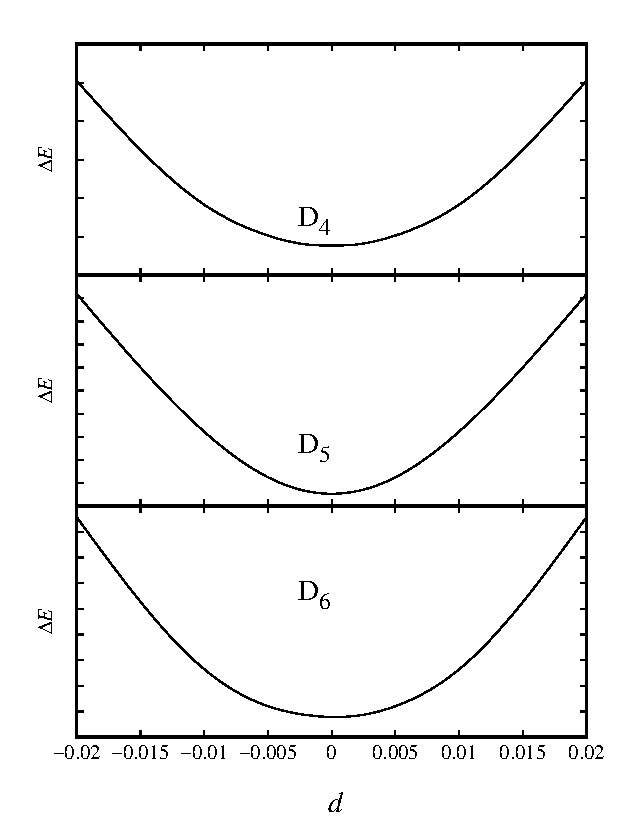
\includegraphics[]{d456_alphaU.eps}
	\caption[Changes in strain energy in $D_4$, $D_5$ and $D_6$]{Changes in the strain energy as a function of strain using distortion matrix~$D_4$~\eqref{eq_D4}, $D_5$~\eqref{eq_D5} and $D_6$~\eqref{eq_D6}.}
	\label{fig_D456}
\end{figure}

\begin{figure}
	\centering
	\includegraphics[]{d789_alphaU.eps}
	\caption[Changes in strain energy in $D_7$, $D_8$ and $D_9$]{Changes in the strain energy as a function of strain using distortion matrix~$D_7$~\eqref{eq_D7}, $D_8$~\eqref{eq_D8} and $D_9$~\eqref{eq_D9}.}
	\label{fig_D789}
\end{figure}


\section{Elastic Parameter Calculation for \textgamma-uranium}\label{appen_bccel}
Applying a small strain ($\delta$) to the equilibrium lattice changes the total energy, and from this information, the elastic parameters are deduced. The distortion of a lattice vector follows the rule $\mathbf{R'} = \mathbf{RD}$. Here, $\mathbf{R}$ is the Bravais lattice vector, $\mathbf{R'}$ is a matrix containing the components of the distorted lattice vectors, and $\mathbf{D}$ is the symmetric distortion matrix.


By symmetry, there are only three independent elastic parameters for a cubic system (\ie, $C_{11}, C_{12}$, and $ C_{44}$).
Elastic parameters are evaluated from the total energy of the crystal, to which volume-conserving orthorhombic $[C'=(C_{11} - C_{12})/2]$ and monoclinic $(C_{44})$ distortions are applied. The relevant distortion matrices are 
%\[\begin{bmatrix}
\begin{equation}
\mathbf{D}_\text{ortho} = \label{eq:ortho}
		\begin{bmatrix}
		1+\delta_o & 0 & 0 \\
		0 & 1-\delta_o & 0 \\
		0 & 0 & \frac{1}{1-\delta_o^2}\\
		\end{bmatrix}
\end{equation}
%\end{bmatrix} \]
and
\begin{equation}
\label{eq:mono}
\mathbf{D}_\text{mono} = \begin{bmatrix}
	1 & \delta_m & 0 \\
	\delta_m & 1 & 0 \\
	0 & 0 & \frac{1}{1-\delta_m^2} \\
\end{bmatrix}.
\end{equation}
The associated total energy change for an orthorhombic distortion is 
\begin{equation}
\label{eq_ortho}
\Delta E = V(C_{11} - C_{12})\delta_o^2 + O(\delta_o^4) .
\end{equation}
For a monoclinic distortion, the energy change is
\begin{equation}
\label{eq_mono}
\Delta E = 2VC_{44}\delta_m^2 + O(\delta_m^4).
\end{equation}

\begin{figure}
	\centering
	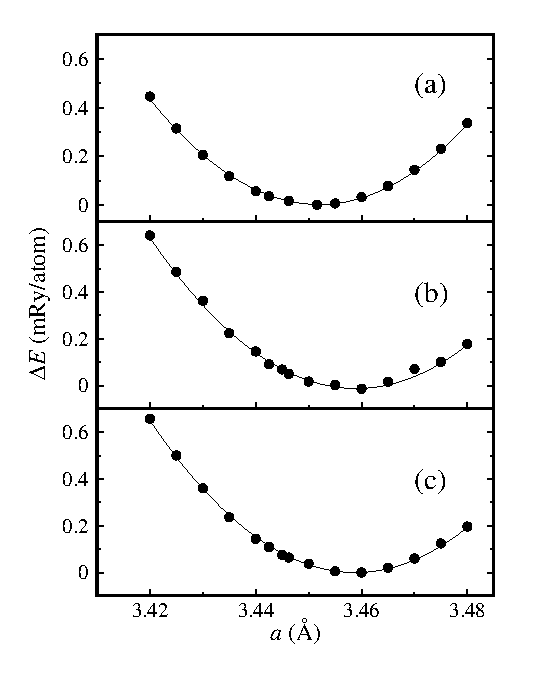
\includegraphics[width=4.25 in]{figure_bulk}
    \caption[Energy as a function of lattice parameters for \textgamma-uranium.]{Energy as a function of lattice parameters for \textgamma-uranium. (a)~Our work~\cite{iasir2020pseudopotential} with a $k$-point mesh of $30\times30\times30$; (b)~Pseudopotential from PS library~\cite{dal2014pseudopotentials, pp1}
 with a $k$-point mesh of $30\times30\times30$; (c)~Pseudopotential from PS library~\cite{dal2014pseudopotentials, pp1}
 with $42\times42\times42$ $k$-point mesh.}
	\label{fig:bulkgamma}
\end{figure}

\begin{figure}
	\centering
	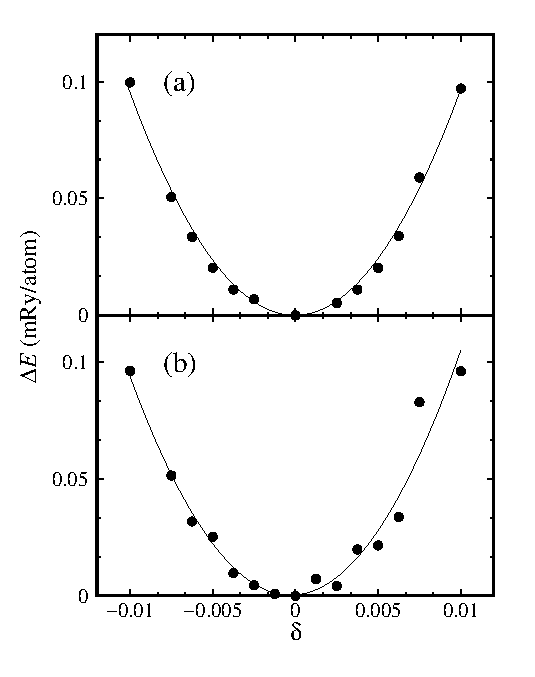
\includegraphics[width=4.25 in]{figure_mono}
    \caption[Changes in the strain energy as a function of strain $(\delta)$ for monoclinic distortions of \textgamma-uranium ]{Changes in the strain energy as a function of strain $(\delta)$ for monoclinic distortions of \textgamma-uranium (Eq.~\eqref{eq:mono} and Eq.~\eqref{eq_mono}). (a)~Our work~\cite{iasir2020pseudopotential}; (b)~Pseudopotential from the PS library~\cite{dal2014pseudopotentials, pp1}. Increasing the $k$-points does not improve the smoothness of plot (b).}
\label{fig:monogamma}
\end{figure}

\begin{figure}
	\centering
	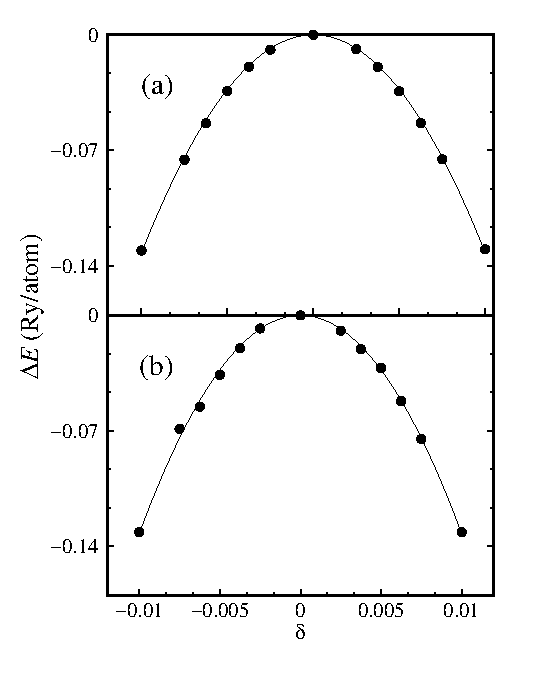
\includegraphics[width=4.25 in]{figure_ortho}
    \caption[Changes in the strain energy as a function of strain $(\delta)$ for orthorhombic distortions of \textgamma-uranium ]{Changes in the strain energy as a function of strain $(\delta)$ for orthorhombic distortions of \textgamma-uranium (Eq.~\eqref{eq:ortho} and Eq.~\eqref{eq_ortho}). (a)~Our work~\cite{iasir2020pseudopotential}; (b)~Pseudopotential from the PS library~\cite{dal2014pseudopotentials, pp1}.}
	\label{fig:orthogamma}
\end{figure}

\end{appendices}


%\bibliographystyle{iopart-num}
\bibliographystyle{apsrev4-1}
\bibliography{abbreviated,comp}
